% Chapter Template

\chapter{Estructura del mutualismo} % Main chapter title
\label{ESTATICA} % Change X to a consecutive number; for referencing this chapter elsewhere, use \ref{ChapterX}

%----------------------------------------------------------------------------------------
%	SECTION 1
%----------------------------------------------------------------------------------------

\section{Propiedades estructurales del mutualismo}

Lorem ipsum dolor sit amet, consectetur adipiscing elit. Aliquam ultricies lacinia euismod. Nam tempus risus in dolor rhoncus in interdum enim tincidunt. Donec vel nunc neque. In condimentum ullamcorper quam non consequat. Fusce sagittis tempor feugiat. Fusce magna erat, molestie eu convallis ut, tempus sed arcu. Quisque molestie, ante a tincidunt ullamcorper, sapien enim dignissim lacus, in semper nibh erat lobortis purus. Integer dapibus ligula ac risus convallis pellentesque 

%-----------------------------------
%	SUBSECTION 1
%-----------------------------------
\subsection{Magnitudes clásicas}

Nunc posuere quam at lectus tristique eu ultrices augue venenatis. Vestibulum ante ipsum primis in faucibus orci luctus et ultrices posuere cubilia Curae; Aliquam erat volutpat. Vivamus sodales tortor eget quam adipiscing in vulputate ante ullamcorper. Sed eros ante, lacinia et sollicitudin et, aliquam sit amet augue. In hac habitasse platea dictumst.

\section{Descripción basada en la descompisión \textit{k-core}}

La \textit{descomposición k-core}\footnote{Utilizamos la expresión original en inglés por ser prevalente en la bibliografía, a pesar de que algunos autores han propuesto traducciones como textit{núcleos de grado k} \cite{herrero2000terminologia} o \textit{k-núcleos} \cite{cardona2006taxonomia, martinez2011aplicacion}} fue utilizada por primera vez por Stefen Seidman para medir la densidad local y la cohesión en redes sociales \cite{seidman1983network}. Dado un grafo no dirigido, un \textit{k-core} es el subgrafo máximo el el que todos sus nodos están conectados con al menos otros $k$ puntos \cite{dorogovtsev2006k}.

\begin{defn} 
Sea un grafo no dirigido $G = \{V, E\}$, donde $V$ y $E$ son los conjuntos de nodos y enlaces respectivamente. Llamamos $deg_G(v)$ al grado del nodo $v$ en el grafo $G$. El subgrafo $M = \{C, E|C\}$ inducido por el subconjunto de nodos $C \subseteq V$ es
un $k$-$core$ si $\forall v \in C: \big( deg_G(v) \geq k \big)$ y $M$ es el subgrafo máximo que cumple la condición. Se denomina $k$-$shell$ al conjunto de nodos del $k$-$core$ que no pertenecen al $k+1$-$core$.
\label{ESTATICA_def_kcore}
\end{defn}

La \textit{descomposición k-core} se ha utilizado de forma habitual como mecanismo de reducción de información para estudiar redes de distinta naturaleza \cite{kitsak2010identification, zhang2010using, barbera2014critical}. El resultado ofrece una visión organizada en capas, con los nodos más centrales en la \textit{shell} de mayor $k$. Esta cifra puede llegar al orden de las centenas en redes grandes. Hasta donde nosotros sabemos, no hay literatura sobre su aplicación al estudio del mutualismo, ya que son redes bipartitas de un tamaño mínimo comparado con los sistemas sociales o tecnológicos a los que se ha aplicado.

Existen diversos algoritmos para llevar a cabo la descomposición en función de las dimensiones de la red\cite{montresor2013distributed}. El más sencillo y válido para el caso de las redes mutualistas, es el algoritmo de podado (\textit{pruning}), que se describe con la ayuda de la figura \ref{fig:ESTATICA_kcore_decomposition_example}, una red bipartita ficticia, con ocho nodos de una clase y siete de la opuesta. A la hora de aplicar el algoritmo resulta irrelevante que la red sea bipartita, pues solo se basa en el número de enlaces y no en la naturaleza de los nodos que conectan.

Se empieza eliminando enlaces de aquellos nodos que solo tienen un enlace, por ejemplo el que une el nodo de color verde número 8 con el de color chocolate número 4. Se sigue realizando la operación mientras queden nodos con un único enlace, hasta que llegue el momento en que todos los nodos restantes tengan dos o más. Los nodos que han quedado desconectados forman la \textit{1-shell}. Repetimos el procedimiento para dos enlaces y así sucesivamente, clasificando todos los nodos en su \textit{shell} correspondiente. En este ejemplo sencillo el $k$ máximo es 3. Nótese que cada nodo pertenece a una $shell$.

\begin{figure}[h!]
\centering
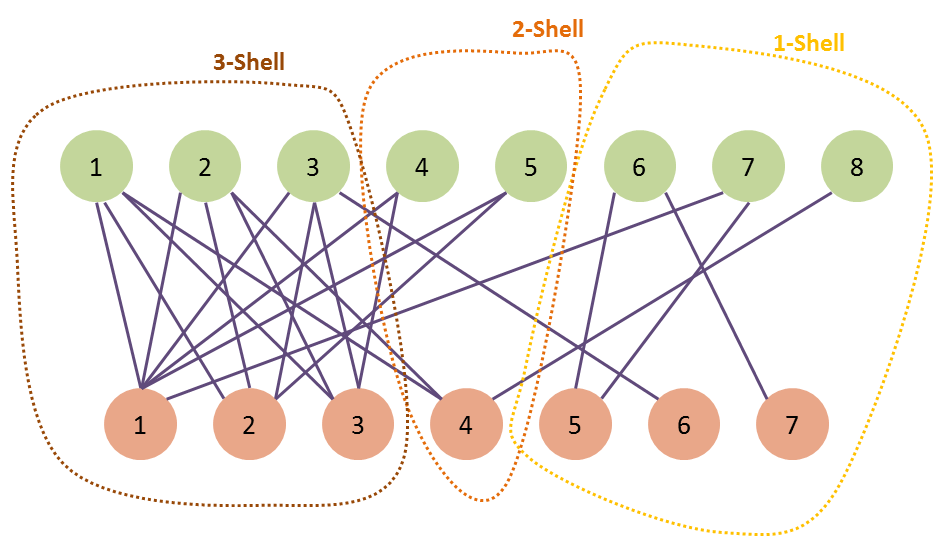
\includegraphics[scale=0.5]{Figures/ESTATICA_kcore_decomposition_example.png}
\caption[PolarExample]{Descomposición \textit{k-core} de una red bipartita ficticia.}
\label{fig:ESTATICA_kcore_decomposition_example}
\end{figure}

Según la definición \ref{ESTATICA_def_kcore}, el  \textit{1-core} es la unión de las tres \textit{shell}, mientras que el \textit{2-core} es la unión de la \textit{2-shell} y la \textit{1-shell}. El \textit{k-core} máximo coincide con la  \textit{k-shell} máxima. 

Como estamos tratando de redes bipartitas, distinguimos dos subconjuntos en cada \textit{k-shell}, el de los nodos de la clase $A$ y el de los de la clase $B$. Los llamaremos $K^{A}_{j}, K^{B}_{j}$, donde  $j$ es el índice de la \textit{k-shell}.
Es posible que uno de ellos sea vacío, es decir, no todas las \textit{k-shell} tienen nodos de ambas clases necesariamente.
Al valor máximo de \textit{k}, lo llamamos $ks_{max}$, que corresponde a \textit{shell} más interna de la red $ks_{max}\equiv C^{A,B}$. Esta nomenclatura simplifica la definición de las \textit{k-magnitudes} que surgen de la red descompuesta siguiendo el procedimiento descrito.


\section{K magnitudes}

Las especies más conectadas de una red mutualista son resistentes a las perturbaciones externas porque el beneficio que reciben depende de múltiples fuentes. Esta parece ser la razón por la que las redes mutualistas tienden al anidamiento, una conexión directa con el centro de la red aumenta las probabilidades de supervivencia. Para medir la 'distancia' desde un nodo cualquiera a la \textit{k-shell} más interna de la clase opuesta, hemos definido el  \textit{$k_{radius}$}.

\begin{defn} 
El \textit{$k_{radius}$} del nodo $m$ de la clase $A$ es el valor medio de la distancia a las especies de $C^B$.

\begin{align*}
\displaystyle
k^A_{radius}m = \frac{1}{\mid C^{B} \mid}\sum\limits_{j \in C^{B}} dist_{mj}  \qquad   m \in A
\stepcounter{equation}\tag{\theequation}\label{kradius}
\end{align*}
\label{ESTATICA_kradius}
\end{defn}

En la fórmula \ref{ESTATICA_kradius} $dist_{mj}$ es el camino más corto de la especie $m$ a cada una de las $j$ especies que forman el conjuto $C^B$. La misma definción es válida para especies de la clase $B$, calculando la distancia media a las especies de $C^A$. El valor mínimo posible de $k_{radius}$ es $1$ para un nodo perteciente a $C^B$ conectado con todas las especies de $C^A$ (y viceversa).

\begin{figure}[h!]
\centering
\includegraphics[scale=0.5]{ESTATICA_red_example.eps}
\caption {Cálculo de \textit{$k_{radius}$} y  \textit{$k_{degree}$} en una red ficticia.}
\label{fig:ESTATICA_red_example}
\end{figure}

La parte superior izquierda de la figura \ref{fig:ESTATICA_red_example} es el esquema de otra red ficticia muy sencilla, con solo siete nodos, tres de la clase $A$ y cuatro de la $B$. La descomposición $k$-$core$ indica que la especie $B4$ es la única de la $1$-$shell$. El resto pertenecen a la $2$-$shell$, que por ser la más interna sirve de base para medir el $k_{radius}$. 

En la parte superior derecha de la imagen, se reproduce el detalle de las conexiones de la especie $A1$, perteneciente a $C^{A}$.  Como está directamente conectada con los tres nodos de $C^{B}$ la el camino más corto a cada uno de ellos es $1$, y en consecuencia \textit{$k^A_{radius}1$} es $1$. En la parte inferior derecha, la especie $A2$ que también pertenece a $C^{A}$ no tiene enlace directo con $B2$, aunque sí con $B1$ y $B3$. El camino más corto, marcado en color violeta, pasa por $B1$ y $A1$, y mide $3$. El \textit{$k^A_{radius}2$} vale $\frac{5}{3}$. En la parte inferior izquierda, vemos el esquema de conexiones de la especie $B4$, que no forma parte de $C^{B}$. Como cabía esperar, su\textit{$k_{radius}$} es mayor, $\frac{7}{3}$. 

Podemos definir una magnitud global, teniendo en cuenta los $k_{radius}$ de todas las especies.

\begin{defn} 
El \textit{$\overline k_{radius}$} de una red se obtiene promediando los ${k}_{radius}$ de todos los nodos, sin importar la clase a la que pertenezcan.

\begin{align*}
\displaystyle
\overline {k}_{radius} = \frac{1}{\mid A \cup B \mid}\sum\limits_{l \in A \cup B} k_{radius}l
\stepcounter{equation}\tag{\theequation}\label{avgkradius}
\end{align*}
\label{ESTATICA_avgkradius}
\end{defn}


A network with all its nodes connected to the innermost core (full-connected or square adjacency matrix) will exhibit $\overline {k}_{radius}=1$ and a network with a triangular adjacency matrix will exhibit  $\overline {k}_{radius}=1.5$. In our example network of Figure \ref{fig:ESTATICA_red_example}, the value is $11/7$. From an intuitive point of view, $\overline {k}_{radius}$ will be small for strongly nested networks. Generalists are very interconnected and specialists have direct ties to higher \textit{k-shells}. On the other hand, a random link distribution means low nestedness and longer paths.

${k}_{radius}$ is a useful magnitude \emph{to measure nestedness} but it not a good measure of centrality. For instance, its value for an isolated specialist linked to the maximum core is low. \emph{To attend this necessity,} we define a second \textit{k-magnitude}, the ${k}_{degree}$:

\begin{align*}
\displaystyle
k^A_{degree}m = \sum\limits_{j} \frac{a_{mj} }{k_{radius}j}  \quad   m \in A, \forall j \in B
\stepcounter{equation}\tag{\theequation}\label{kdegree}
\end{align*}

\noindent where $a_{mj}$ is the element of the interaction matrix that represents the link. So the $k_{degree}m$ is the sum of the inverse of $k_{radius}$ for each node linked to $m$. A node of the innermost shell will have a high degree, whereas specialists have only one or two links and so a low $k_{degree}$. In the example of Figure \ref{fig:red_example}, this magnitude is $1+3/5+3/5 = 11/5$ for node $B3$, while only $3/7$ for node $B4$. This magnitude reminds the definition of the \textit{Harary index} \cite{plavvsic1993harary} but only considering paths to the nodes in the core.


\subsection{Algoritmo de destrucción basado en \textit{k-shell}}

Nunc posuere quam at lectus tristique eu ultrices augue venenatis. Vestibulum ante ipsum primis in faucibus orci luctus et ultrices posuere cubilia Curae; Aliquam erat volutpat. Vivamus sodales tortor eget quam adipiscing in vulputate ante ullamcorper. Sed eros ante, lacinia et sollicitudin et, aliquam sit amet augue. In hac habitasse platea dictumst.

\section{Resultados}

Nunc posuere quam at lectus tristique eu ultrices augue venenatis. Vestibulum ante ipsum primis in faucibus orci luctus et ultrices posuere cubilia Curae; Aliquam erat volutpat. Vivamus sodales tortor eget quam adipiscing in vulputate ante ullamcorper. Sed eros ante, lacinia et sollicitudin et, aliquam sit amet augue. In hac habitasse platea dictumst.

\section{Conclusiones}

Nunc posuere quam at lectus tristique eu ultrices augue venenatis. Vestibulum ante ipsum primis in faucibus orci luctus et ultrices posuere cubilia Curae; Aliquam erat volutpat. Vivamus sodales tortor eget quam adipiscing in vulputate ante ullamcorper. Sed eros ante, lacinia et sollicitudin et, aliquam sit amet augue. In hac habitasse platea dictumst.
